\documentclass[12pt,a4paper]{article}
\usepackage[utf8]{inputenc}
\usepackage[left=20mm,top=20mm,bottom=30mm]{geometry}
\usepackage{graphicx}
\usepackage{alltt}
\usepackage{color, colortbl}

\definecolor{lightgray}{gray}{0.9}
\definecolor{darkgray}{gray}{0.8}

\newcommand{\tab}{\hspace*{2em}}

\begin{document}
\title{Prosjektplan \\ for \\ SkyHiGH Feide}
\author{Fredrik Magnussen, Håkon Tvedt og Morten Hanssen Singstad}
\maketitle
\begin{center}
	
\includegraphics[scale=1]{logo.png}
\end{center}

\newpage
\tableofcontents

\newpage
\section{Mål og rammer}
\subsection{Bakgrunn}
Opphavet til dette prosjektet er at Høgskolen i Gjøvik skal ha en skyløsning stående på skolen, som kan kjøre VM-er til forskjellige fag og andre som eventuelt trenger VM i henhold til skolen. \newline \newline
Openstack er en opensource løsning på for VM-system. Teknologien benytter seg av å samarbeide mellom flere forskjellige prosjekter som kontrolleres gjennom maskinytelse, lagring og nettverksressurser. Dette kjøres gjennom et datasystem som f.eks. et “rack” med maskiner. Her får man tilgang til å kunne administrere oppsettet av infrastruktur som man produserer med Openstack og valgte installasjoner til Openstack. Et dashboard som gir muligheter til brukere å konfigurere VM-er med ønskede ressurser.
(Informasjon fra [1]Referanser) \newline \newline
VM-er blir brukt i forskjellige fag på HiG. Dette for å spare plass, nettverk, tilkoblinger, ressurser og økonomi. For at dette skal kunne brukes i undervisning så er det nødt til å være enkelt brukergrensesnitt for oppsett at VM-laber. Systemet er også nødt til å være redundant og stabilt, dette med tanke på at man kan ikke miste data som man har jobbet med gjennom semesteret. \newline \newline
Innloggingen til systemet er hovedmålet for denne oppgaven. Den skal implementeres med Feide, dette for at det skal være enkelt for brukerne og logge inn med allerede eksisterende brukernavn og passord. (Brukerne blir mer fornøyd med tanke på at de slipper å huske flere innloggingsinformasjoner).

\subsection{Prosjektmål (Effektmål og resultater)}
Målet for SkyHiGH, er at vi skal kunne ha en fungerende og stabilt oppsett av Openstack som kjører skyløsningssystem i et rack. Med implementert \newline \newline
\textbf{Effektmål:}\newline
Vi skal få installeringen av Openstack til å bli automatisert. Ikke bruke tid på å måtte gjøre kommandoer og svare på spørsmål i henhold til installasjonene. Autentiseringen skal skje med Feide.
\begin{description}
	\item[\tab •] Automatisering av backup og installasjoner for raskere gjennoppretting av system og ressursbesparelse. 
	\item[\tab •] Implementere Feide for å kunne bruke allerede eksisterende brukernavn og passord for brukeren.
	\item[\tab •] Monitoring av hele systemet for vedlikeholdelse og systemvarslinger.
\end{description}
\textbf{Resultatmål:}\newline
Tilpasse OpenStack-infrastrukturen SkyHiGh til FEIDE-autentisering. Utvide og teste
funksjonaliteten for realisering av virtuelle laboratorier i siste versjon av OpenStack Folsom.
\begin{description}
	\item[\tab •] Enklere autentisering for brukerne.
	\item[\tab •] Enklere vedlikeholdelse, automatiserte varslinger og overvåking.
	\item[\tab •] Stabil og sterkere ytelsesmessig løsning som kan erstatte dagens VM-løsning på HiG.
\end{description}

\section{Omfang}
\subsection{Oppgavebeskrivelse}
SkyHiGh er en privat sky-løsning som ble utviklet i to bacheloroppgaver våren 2012, hvorav den ene er omtalt på [2] Referanser. \newline \newline
Denne oppgaven går ut på å fortsette der SkyHiGh Adm-gruppen endte opp. Det betyr
videreutvikling med tanke på integrering mot HiGs brukerhåndtering og autentisering (FEIDE) og
tilpasse modulen utviklet i forrige bacheloroppgave til ny versjon, samt teste og videreutvikle denne slik at SkyHiGh blir et skritt nærmere produksjonsstatus. Målet er at SkyHiGh lett skal kunne realisere virtuelle laboratorier for undervisning og forskning. Trinnvis består oppgaven av:
\begin{description}
	\item[\tab •] Sette seg inn i SkyHiGh Adm og I/O oppgavene
	\item[\tab •] Sette opp SkyHiGh løsningen og oppdatere denne til siste versjon av OpenStack
	\item[\tab •] Utrede og realisere rollebasert identitetshåndtering og tilhørende FEIDE-autentisering
	\item[\tab •] Oppdatere og videreutvikle SkyHiGh Adm-modulen
	\item[\tab •] Teste opprettelse og stabilitet av ulike virtuelle scenarier
\end{description}

\subsection{Avgrensning}
Siden denne oppgaven er ganske stor, så har vi tenkt å fokusere på det viktigste; Det å sette opp og oppdatere løsningen til siste versjon av OpenStack, som er folsom. Vi må også implementere løsningen fra SkyHiGh adm oppgaven, så vi får en helt up-to-date og fungerende løsning. Deretter kommer implementasjonen av FEIDE-løsningen. Vi skal også prøve og automatisere/skripte disse løsningene, så det blir enklere å sette opp senere ved eventuell utskifting av maskinvare/utvidelse av løsningen. Vi tenker også at det kan være greit å sette opp overvåking for å holde kontroll på belastningen. 

\section{Prosjektorganisering}
\subsection{Ansvarsforhold og roller}
\textbf{Oppdragsgiver og veileder}
Oppdragsgiveren/kunden er førsteamanuensis Erik Hjelmås ved Høgskolen i Gjøvik. Erik kommer til å bistå oss mye med både fagelig og teknisk hjelp. Veilederen/Scrum Master er førsteamanusis Hanno Langweg. Han vil bistå oss mye med hvordan vi skal jobbe i prosjektet og komme med innspill angående løsninger. \newline
\textbf{Prosjektleder}
Morten Singstad ble valgt som prosjektleder for gruppa. Dette ansvaret består av å løse eventuelle konflikter som vi ikke har løst i fellesskap. Det er også prosjektlederens overordnede ansvar for at frister blir holdt. \newline
\textbf{Webansvarlig}
Webansvarlig på gruppa er Fredrik Magnussen. Han skal opprette, designe og vedlikeholde websiden. Resten av gruppa skal også ha et ansvar for å opprettholde at websiden blir brukt regelmessig til oppdateringer og lignende. \newline
\textbf{Kontaktperson}
Kontaktpersonen er også prosjektleder (Morten Hanssen Singstad). Kontaktpersonen skal ha hovedsakelig kontakt med oppdragsgiver og veileder, for å avtale møter. De andre på gruppa kan også ta kontakt med oppdragsgiver og veileder vis det blir behov for dette. Kontakt med andre resursser kan deligeres til andre gruppemedlemmer.

\subsection{Rutiner og regler i gruppen}
Gruppa har satt av tid til å jobbe med prosjektoppgaven på mandager, torsdag og fredag fra 08.00 til 16.00. Vi kan gå over de fastsatte tidsrammene hvis nødvendig. Vi skal også prøve å jobbe så mye som mulig mellom andre fag hvis mulig. Helgene er i utgangspunktet fridager, men kan hvis nødvendig, brukes til å jobbe med prosjektet. Gruppens øverige regler ligger på punkt 9.

\subsection{Verktøy}
Til å skrive oppgaven så bruker vi Texmaker som også genererer dokumentet til pdf. Dette har vi koblet opp mot github som fungere som ett repository. Vi har også backup av denne i Dropbox. Til samskriving av tekst som skal inn i  LaTeX-dokumentene, så bruker vi Google Drive, vi gjør dette for å minske sjansen for at vi skriver over hverandre. Det hjelper oss med at vi vet hva de andre skriver, sånn at vi ikke skriver om det samme. Til websiden så har vi planlagt å bruke wordpress. Til prosjektstyringsverktøy så bruker vi Trello. Vi kommer også til å bruke Vmware workstation 9, Ubuntu 12.10, Openstack falsom til diverse testing og utvikling. For å lage gantt skjema så bruker vi gantto.com.

\section{Planlegging, oppfølging og rapportering}
\subsection{Hovedinndelinger av prosjektet}
Før vi får startet ordentlig så er vi nødt til å flytte racket, serverne få opp strøm og internett-tilgang til serverrommet som vi er tildelt. I mellomtiden så jobber vi med å gjøre ferdig prosjektplanen, sette opp VM for å teste installasjon av openstack og Ubuntu 12.10 Server. Vi skal også lese og forstå hva Adm-gruppen gjorde, samt lese om Feide. \newline \newline
Da kan vi få startet med å dele inn prosjektet. Først vil vi få installert serveros-et ved å bruke Preseed. Deretter så skal vi få laget automatiserte installasjoner av de forskjellige nodene som trengs i Openstack (Controller node, Network node og Compute nodene). \newline \newline
Når racket er klart til å brukes så skal vi sette opp infrastructuren i henhold til arkitekturen. For at vi skal ha full tilgang til racket så skal vi sette opp serverne med tilgang gjennom KVM. \newline \newline
Deretter så setter vi opp et basic fungerende Openstack-miljø på serverne med automatisert installering. Vi skal også få opp automatisert backup og mulighet for rollback. Deretter skal vi implementere og sy sammen SkyHiGh Adm delen med den nye Openstack Folsom. Når dette fungerer skal vi installere resten av nodene. \newline \newline
Når vi har et fungerende Openstack-miljø skal vi begynne å implementere Feide autentisering. Hvis vi har et fungerende produkt og tid til overs, skal vi se på løsning for å overvåke.

\subsection{Plan/krav for statusmøter og beslutningspunkter}
Ved at vi bruker Scrum som utviklingsmodell så blir planleggingen gjort utifra den. 
\begin{description}
	\item[\tab  •] Product backlog, Sprint backlog, Sprint, Dagsmøter, Sprintmøter og deretter Ferdig modul.
\end{description}
\textbf{Product backlog:}
\tab Slutt produktet som er bestilt av arbeidsgiver deles opp i “stories” som vil tilsvare “product backlog”-moduler. Disse er utarbeidet i henhold til møter med arbeidsgiver, angående hvordan sluttproduktet skal fungere og hvilke krav for brukergrensesnitt det skal være. \newline
\textbf{Sprint backlog:}
“Product backlog story” blir delt opp i mindre arbeidsoppgaver som kan fordeles utover sprint-en og dagsarbeid.
Sprint: En sprint har vi satt til å være en uke. Her jobber vi med sprint backloggen og det forventes å ha ferdig modul innen endt sprint. \newline
\textbf{Dagsmøter:}
Her diskuteres hva som er gjort, hva som skal gjøres og arbeidsfordeling. Skal ikke overskride 30 minutter. \newline
\textbf{Sprintmøte:}
Møte inneholder scrumleder/veileder, arbeidsgiver og scrumteam. Status på “product backlog”-modulen. Legger fram det som er gjort for arbeidsgiver og tar imot kritikk og forslag til endringer. Hvis modulen er ferdig, vis en demo og presenter hvilken ny “product backlog story” skal vi jobbe med. Hvis modulen ikke er ferdig trengs det en ny sprint på foregående modul.

\subsection{Ressursbehov}
Siden produktet blir satt i produksjon, så trenger vi et oppsett som kan fungere og vare en stund. Med dette vil ressursbehovet være 8 servere. 1 til controller- og network node, 5 til compute noder, 2 til lagring og 1 switch. Og siden vi ikke har full tilgang til utstyret, trenger vi også en KVM-console og KVM-switch.

\section{Organisering og kvalitetssikring}
For at vi skal få et best mulig produkt. Så må vi ha en god plan for hvordan vi skal jobbe, vi setter oss standarder for hvordan og når vi gjør dokumentasjoner, rapporter, typologi og kodesyntax.
\subsection{Dokumentasjon, standardbruk og kildekode}
Rapportskriving av arbeid vil skje løpende og vil hjelpe med å kunne forsklare kunden hva vi har gjort og hvordan. \newline \newline
Dokumentasjon ligger under det samme, men dette må et mye grundigere nivå. Her er det snakk om dokumentering med en samling av kodelinjer, dokumentere funn, løsninger og hvordan vi bruker forskjellige oppsett. Dette gjør vi for at vi ikke skal bruke unødvendig krefter på tid og frustrasjon ved å forstå hva de andre på gruppen har gjort, samt hva vi selv gjorde for lenge siden. \newline \newline
Siden vi bruker Openstack som kjører på Apache 2.0 lisens så følger vi standarder til Apache 2.0.

\newpage
\subsection{Risikoanalyse}
\begin{table}[h]
	\begin{tabular}[Figur 1]{| p{3cm} | p{3cm} | p{5cm} | p{5cm} |}
		\hline \rowcolor{lightgray} \textbf{Beskrivelse} & \textbf{Sannsynlighet} & \textbf{Konsekvens} & \textbf{Løsning} \\
		\hline \rowcolor{darkgray} Sykdom blant teamet & lav & Mangel på arbeidskraft & Tilrettelegging av arbeidsforhold for den syke. \\
		\hline \rowcolor{lightgray} Tap av data ved tekniske feil eller menneskefeil (skrive over eller sletter feil). &	lav/middels &	Detter langt tilbake i arbeid og kan resultere i at  oppgaven blir veldig redusert. Mye ekstra jobb. & Kontinuerlig backup(automatisert) og repository på det vi skriver. \\
		\hline \rowcolor{darkgray} Mangel på kompetanse &	middels & Bruker lengre tid på å få til, rekker ikke tidsfrister og kan resultere i dårlig utførelser. & Les seg opp, samarbeide for å forstå. Få  informasjon fra noen med kompetanse. \\
		\hline \rowcolor{lightgray} Dårlig tidsplanlegging & høy & Mer jobb en det vi trodde. Sluttprodukt kan risikere å ikke bli ferdig. & Ikke undervurdere mengde arbeid og mengden tid som må brukes. \\
		\hline \rowcolor{darkgray} Endringer som er ødeleggende &	middels/høy	 & Tap av data, konfigurasjon og oppsett. & Backup, automatisert installasjon, mulighet for rollback. \\
		\hline \rowcolor{lightgray} Dårlig dokumentering & lav/middels & Vanskelig å rette opp feil. Hvis systemet må settes opp på nytt, er dokumentering viktig for å se hva vi har gjort. & Passe på hverandre i forhold til dokumentasjon. Ofte påminning.
	\end{tabular}
\end{table}

\newpage
\section{Plan for Gjennomføring}
\subsection{Fremdriftsplan}
\begin{figure}[h]
	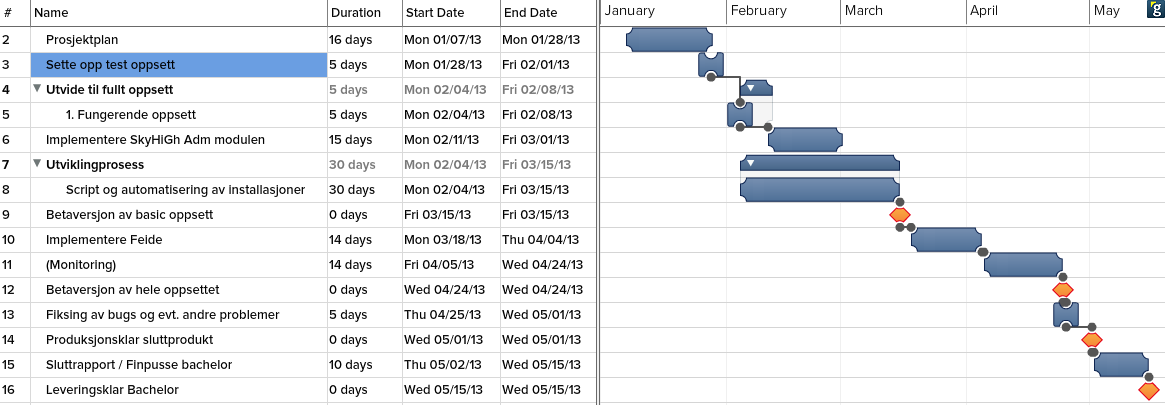
\includegraphics[height=100mm,width=170mm]{bachelorgantt.png}
\end{figure}

\section{Prosjektavtale}

\section{Referanser}

\newpage
\section{Grupperegler}
\begin{flushright}
	\begin{figure}[h]
		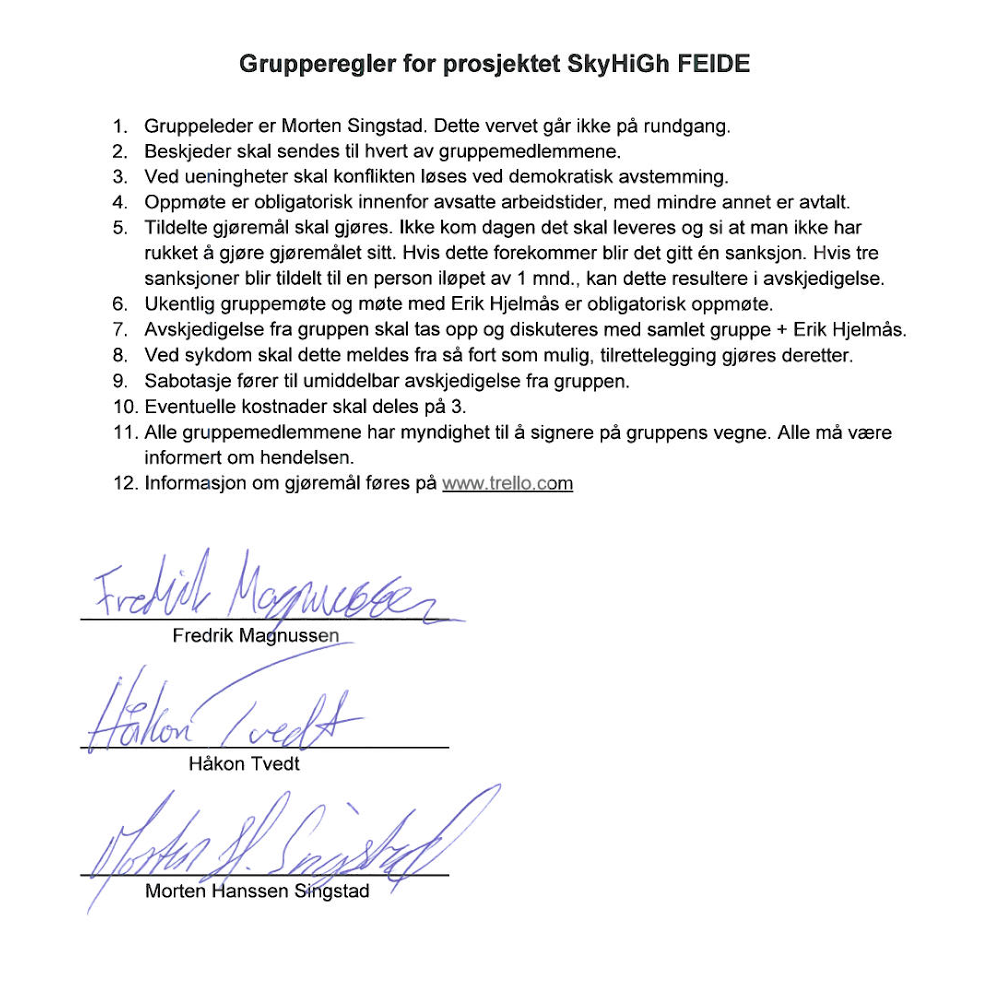
\includegraphics[width=150mm,height=150mm]{grupperegler.png}
 	\end{figure}
\end{flushright}

\end{document}
